\documentclass{article}
\usepackage[ampersand]{easylist}
\usepackage{amsmath}
\usepackage[inline]{enumitem}
\usepackage{lscape}
\usepackage{graphicx}
\graphicspath{ {C:/Users/ustjo/Desktop/Investing/Stocks/canslim/weeklyStockScanner/Figures/} }
\begin{document}
\title{Weekly Stock Scanner Result \\ 20180115 to 20180128}
\author{KAI YIN, CHAN}
\maketitle

\section{Portfolio}
14 shares of PFG @ 69 with an unrealized profit of 69.2 on 23/01/2018

\subsection{Action}
SL modified from 67.96 to 69
TP: 79.35 SL: 69.0

\section{Stocks that passed scanning}

There are 6 out of 4823 stocks passed the scanning.  They are:
% Table generated by Excel2LaTeX from sheet 'Sheet1'
\begin{table}[htbp]
  \caption{Stocks that passed scanning}
    \begin{tabular}{lllll}
    	\textbf{Symbol} & \textbf{Name} & \textbf{Sector} & \textbf{Market Cap} & \textbf{Exchange} \\
    	AQN   & Algonquin Power \& Utilities Corp. & Public Utilities & \$4.71B & NYSE \\
    	EPAM  & EPAM Systems, Inc. & Technology & \$5.74B & NYSE \\
    	NTRI  & NutriSystem Inc & Consumer Services & \$1.63B & Nasdaq \\
    	NVEE  & NV5 Global, Inc. & Consumer Services & \$585.66M & Nasdaq \\
    	PFG   & Principal Financial Group Inc & Finance & \$20.58B & Nasdaq \\
    	THO   & Thor Industries, Inc. & Consumer Non-Durables & \$8B  & NYSE \\
    \end{tabular}%
    \label{tab:addlabel}%
\end{table}%

\subsection{Actions}
NVEE shows a double bottom pattern with buy point at 54.1 and buy range to 56.79. please see Table \ref{data} and Table \ref{checking} as well as Figure \ref{NVEE}.

Set stop limit at 54.10. Take profit at 62.25. Take loss at 51.4.

\begin{figure}
\caption{NVEE Double Bottom}
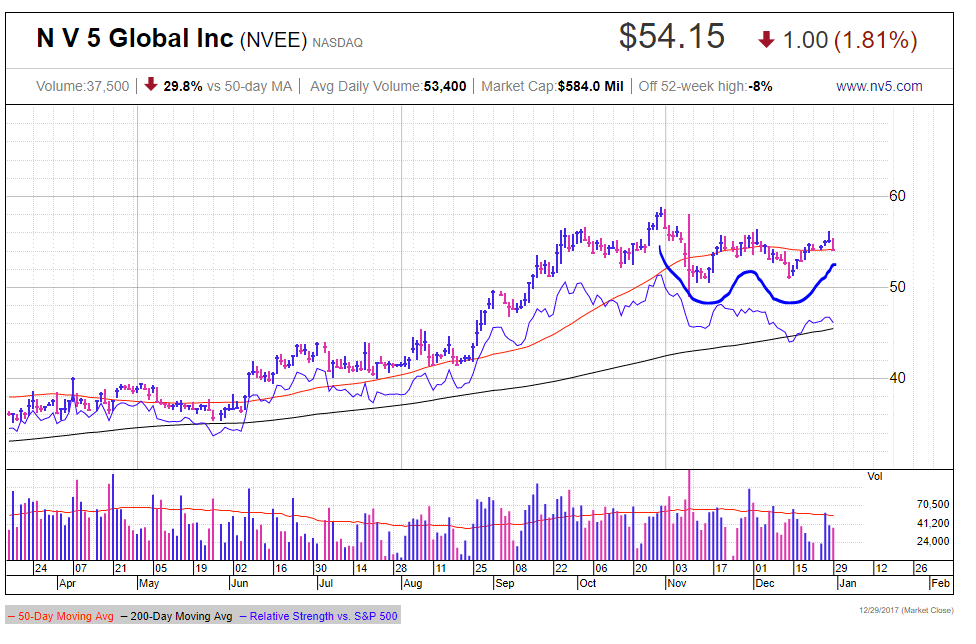
\includegraphics[width = \textwidth]{NVEE_20180101.png}
\label{NVEE}
\end{figure}

% Table generated by Excel2LaTeX from sheet 'For Latex'
\begin{table}[htbp]
	\centering
	\caption{Double bottom data}
	\begin{tabular}{rlr}
		\multicolumn{1}{l}{Data} &       &  \\
		\multicolumn{1}{l}{Left} & Date  & 43040 \\
		& Price & 56.6 \\
		\multicolumn{1}{l}{Bottom 1} & Date  & \multicolumn{1}{l}{N.A.} \\
		& Price & 52.05 \\
		\multicolumn{1}{l}{Middle} & Date  & \multicolumn{1}{l}{N.A.} \\
		& Price & 54.09 \\
		\multicolumn{1}{l}{Bottom 2} & Date  & \multicolumn{1}{l}{N.A.} \\
		& Price & 51.85 \\
		\multicolumn{1}{l}{Right} & Date  & 43097 \\
		& Price & 55.15 \\
	\end{tabular}%
	\label{data}%
\end{table}%

% Table generated by Excel2LaTeX from sheet 'For Latex'
\begin{table}[htbp]
	\centering
	\caption{Checkings}
	\begin{tabular}{lllr}
		Checkings &       &       &  \\
		& Actual & Rquired & \multicolumn{1}{l}{Passed} \\
		Bottom 2 compared with Bottom 1 & N.A.  & B2 < B1 & TRUE \\
		Base Length & \multicolumn{1}{r}{8.142857} & \multicolumn{1}{r}{7} & TRUE \\
		Base Correction & \multicolumn{1}{r}{-8.39223} & \multicolumn{1}{r}{-30} & TRUE \\
		W shape & W     & W     & TRUE \\
		Apex above 10 days moving average & Y     & Y     & TRUE \\
	\end{tabular}%
	\label{checking}%
\end{table}%

\section{Appendix}
% Table generated by Excel2LaTeX from sheet 'Sheet1'
\begin{table}[htbp]
  \caption{Quarterly EPS}
   \begin{tabular}{lrrrrr}
   	\textbf{Symbol} & \multicolumn{1}{l}{\textbf{DEPS Q1}} & \multicolumn{1}{l}{\textbf{DEPS Q2}} & \multicolumn{1}{l}{\textbf{DEPS Q3}} & \multicolumn{1}{l}{\textbf{DEPS Q4}} & \multicolumn{1}{l}{\textbf{DEPS Q5}} \\
   	AQN   & 0.14565 & 0.11593 & 0.06738 & 0.1587 & 0.05496 \\
   	EPAM  & 0.77195 & 0.68114 & 0.4387 & 0.46387 & 0.48593 \\
   	NTRI  & 0.49596 & 0.80895 & 0.24822 & 0.29498 & 0.26644 \\
   	NVEE  & 0.54814 & 0.40275 & 0.21177 & 0.31282 & 0.32877 \\
   	PFG   & 2.76424 & 1.0574 & 1.19323 & 1.08755 & 1.05765 \\
   	THO   & 2.43109 & 2.26195 & 2.10833 & 1.22831 & 1.49404 \\
   \end{tabular}%
   \label{tab:addlabel}%
\end{table}%

% Table generated by Excel2LaTeX from sheet 'Sheet1'
\begin{table}[htbp]
  \caption{Quarterly Sales}
    \begin{tabular}{lrrrrr}
    	\textbf{Symbol} & \multicolumn{1}{l}{\textbf{TR Q1}} & \multicolumn{1}{l}{\textbf{TR Q2}} & \multicolumn{1}{l}{\textbf{TR Q3}} & \multicolumn{1}{l}{\textbf{TR Q4}} & \multicolumn{1}{l}{\textbf{TR Q5}} \\
    	AQN   & 443.316 & 453.223 & 557.917 & 310.234 & 221.277 \\
    	EPAM  & 377.523 & 348.977 & 324.651 & 313.525 & 298.293 \\
    	NTRI  & 158.149 & 194.894 & 212.677 & 108.947 & 124.571 \\
    	NVEE  & 91.263 & 83.736 & 64.059 & 63.022 & 60.091 \\
    	PFG   & 4644.4 & 3192.5 & 3078.2 & 3542.8 & 2829.3 \\
    	THO   & 2231.668 & 1934.672 & 2015.224 & 1588.525 & 1708.531 \\
    \end{tabular}%
    \label{tab:addlabel}%
\end{table}%

% Table generated by Excel2LaTeX from sheet 'Sheet1'
\begin{table}[htbp]
  \caption{EPS, Cash Flow, Sales TTM}
   \begin{tabular}{lrrr}
   	\textbf{Symbol} & \multicolumn{1}{l}{\textbf{EPS TTM}} & \multicolumn{1}{l}{\textbf{CashTTM}} & \multicolumn{1}{l}{\textbf{RetTTM}} \\
   	AQN   & 0.48766 & 1.17454 & 8.0051 \\
   	EPAM  & 2.35566 & 2.86176 & 14.79861 \\
   	NTRI  & 1.84811 & 2.34781 & 50.49423 \\
   	NVEE  & 1.47548 & 2.55247 & 10.3356 \\
   	PFG   & 6.10242 & 7.539723 & 15.67812 \\
   	THO   & 8.02968 & 9.81829 & 28.1694 \\
   \end{tabular}%
   \label{tab:addlabel}%
\end{table}%%

% Table generated by Excel2LaTeX from sheet 'Sheet1'
\begin{table}[htbp]
  \caption{Annual EPS}
    \begin{tabular}{lrrrrr}
    	\textbf{Symbol} & \multicolumn{1}{l}{\textbf{DEPS Y1}} & \multicolumn{1}{l}{\textbf{DEPS Y2}} & \multicolumn{1}{l}{\textbf{DEPS Y3}} & \multicolumn{1}{l}{\textbf{DEPS Y4}} & \multicolumn{1}{l}{\textbf{DEPS Y5}} \\
    	AQN   & 0.43974 & 0.42146 & 0.31582 & 0.27647 & 0.08005 \\
    	EPAM  & 1.86538 & 1.62459 & 1.40027 & 1.28198 & 1.17304 \\
    	NTRI  & 1.19056 & 0.88559 & 0.65804 & 0.25407 & -0.102 \\
    	NVEE  & 1.21666 & 1.17685 & 0.875 & 0.69548 & 0.52032 \\
    	PFG   & 4.49778 & 4.05805 & 3.71979 & 2.95003 & 2.57523 \\
    	THO   & 7.09373 & 4.90625 & 3.79178 & 3.28918 & 2.85559 \\
    \end{tabular}%
    \label{tab:addlabel}%
\end{table}%

% Table generated by Excel2LaTeX from sheet 'Sheet1'
\begin{table}[htbp]
  \caption{Consensus Earnings and Institutional Ownership}
    \begin{tabular}{lrrrr}
    	\textbf{Symbol} & \multicolumn{1}{l}{\textbf{CEPS Y1}} & \multicolumn{1}{l}{\textbf{CEPS Y2}} & \multicolumn{1}{p{4.215em}}{\textbf{Number Institutional Shareholders}} & \multicolumn{1}{p{4.215em}}{\textbf{Institutional Ownership}} \\
    	AQN   & 0.705 & 0.745 & 298   & 0 \\
    	EPAM  & 3.42  & 4.165 & 690   & 136 \\
    	NTRI  & 1.95  & 2.268 & 549   & 168 \\
    	NVEE  & 2.335 & 2.825 & 225   & 94 \\
    	PFG   & 5.215 & 5.63  & 1420  & 91 \\
    	THO   & 6.75  & 9.123 & 991   & 132 \\
    \end{tabular}%
    \label{tab:addlabel}%
\end{table}%

\end{document}
